\documentclass{../../myassignment}

\exercisesheet{Oblig 1}{Samspill og interessente}
\courselabel{IN1030}

\begin{document}

	For disse oppgavene har jeg valgt å utforske Vy, siden det er et system jeg er inneforstått med hvordan bør fungere, da jeg bruker tjenestene dems i ny og ne. 

	\subsection*{Oppgave 1 --- Rike bilder}
	\paragraph*{a)}
	\begin{answer}
		En sluttbruker i dette systemet kunne vært Pavel Durov, en 35 år gammel utvikler som reiser mye rundt i verden, og som tar stor pris på kvalitet og personværn. Selv om han ikke direkte bor i Norge, vil han nok likevel ønske å bruke systemene en del. I og med at ikke han har en rutinert hverdag, spesiselt ikke i Norge (der Vy eksisterer), vil han nok ha noen andre krav en de noen som reiser frem og tilbake mellom hjem og skole hver dag. 

		Ut i fra dette, la oss si at Durov vil bruke systemet en gang i året. Han planlegger nok reisen før han kommer hit, og ønsker derfor å ha forbredt tilgang til Vy sine servicer fullstendig før han kommer til landet, for å slippe å tenke på dette når han først er fremme. Han er litt sær når det kommer til telefonbruk, da han ikke er glad i systemer han ikke er kjent meg, og ønsker nok å kunne ha tilgang til billettene sine uten å måtte ha nett-tilgang, eller å måtte utgi personlig informasjon om seg selv. 

	\end{answer}

	\paragraph*{b)}
	\begin{answer}
		Det er flere åpenbare interessenter i denne situasjonen. For det første, som vi allerede har nevnt, har vi kundene/sluttbrukerene, som vil flytte seg fra A til B, evt. videre til C. Det er jo det som er hovedproduktet/målet i denne situasjonen. 

		Videre er det lett å tenke på lederene av Vy, deriblant Dag Mejdell og Geir Isaksen. I og med at Vygruppen AS er eid av Samferdselsdepartementet har staten en direkte kobling til selskapet, og er dermed en tett interessent. Selv om ikke staten hadde hatt eid selskapet ville den vært en interessent, siden Norge ønsker å tilby det beste tilbudet til folket, innenfor økonomiens muligheter. 

		Når disse er nevnt, kan vi ikke utelukke andre transport-selskap i området. Blant disse har vi først og fremst Ruter (i Oslo og Akershusområdet), og privatselskap som Flybussen(e). Ruter og Vy sammarbeider godt, med å dele områder for å bidra til beste felles service.

	\end{answer}

	\paragraph*{c)}
	\begin{answer}
		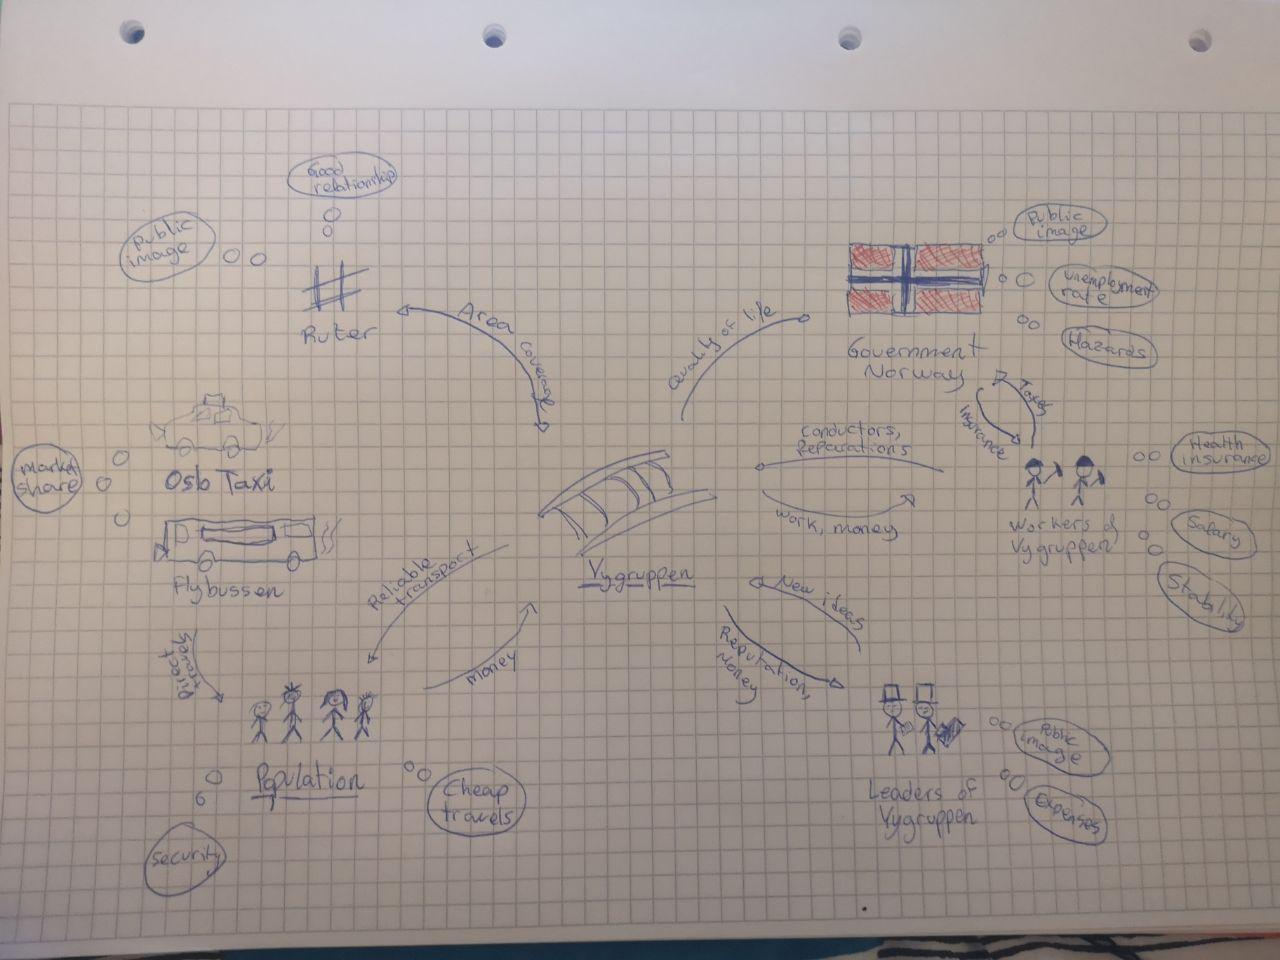
\includegraphics[scale=0.4]{vygruppenrelationships.jpg}

	\end{answer}

	\paragraph*{d)}
	\begin{answer}
		Det er viktig å vite hvilke konflikter og motsigelser som finnes mellom interessentene, da det kan skape problemer om ikke begge/alle partiene er kommet til en felles avtale/evighet. Vi kan se en klar konflikt mellom arbeidere og ledelsen av Vy, siden arbeiderene ønsker høyere lønn, mens ledelsen ønsker lavere utgifter. Tilsvarende vet vi at befolkningen ønsker billige reiser, mens ledelsen ønsker å øke inntektene. Når det gjelder arbeiderene er det relativt lett å komme til en enighet, mens når det kommer til befolkningen er dette noe som må tilpasses over tid, både for å bli kjent med markedet, og for å tilpasse seg den økonomiske inflasjonen. 


	\end{answer}

	\paragraph*{e)}
	\begin{answer}
		Å kartlegge trusler, strukturer, og prosesser er en ting, og det er mange måter å gjøre dette på. Det jeg ikke har forstått helt er hvilken forskjell man gjør, bevisst, for å ``lage en rask og enkel versjon'', enn når en lagger en fullstendig versjon. I en brainstorming-fase gir ikke dette noen mening for meg, men jeg kan forstå det i en langvarig prosess, der man går gjennom planleggingsdokumentene atter igjen for å revidere dem. Denne type ``kart'' er jo mer en slags idé-projeksjon, som jeg ser det for meg, og ikke et direkte planleggingsverktøy.

		Det andre jeg lurer på er hvordan man får folk til å ønske å sette av tid til å planlegge ting på en fornuftig måte. Alt for ofte opplever man at man må starte å produsere før man har noen faktisk plan, mens andre ganger kan vi drive med research og perfeksjonering til verden er gått under. Jeg føler selv jeg har en fornuftig balanse for dette i underbevisstheten, men hvordan kan slikt bli behandlet profesjonelt, og rasjonelt, i en større sammenheng enn som standalone developer?

	\end{answer}

	\pagebreak

	\subsection*{Oppgave 2 --- Samspill}

	\paragraph*{a)}

	\begin{problem}
		Disse endringene er vanskelige fullt ut å planlegge, styre og forutse.
	\end{problem}

	\begin{answer}
		For å svare på dette spørsmålet kan vi jo bare gå i historieboka: ARPANET ble laget som en militer ressurs for å kommandere og ta valg. Nå er det forgjengeren til dagens Internett. FaceMash, nåværende Facebook, var opprinnelig bare en platform for universitetsstudenter for å date. Nå er det en av de største informasjonssamlerene i verden. Side om side til Google, vil jeg si. 

		Google sin guideline om etiske beslutninger sa tidligere ``Don't be evil.'' Nå sier den ``Do the right thing''. Grunnen til dette er at det er vanskelig å objekit definere hva som er ``ondt'', uten noen form for bias. Noen mener også at Google i seg selv er ondsinnet siden de tracker data.

		Poenget med disse eksemplene er at endringer skjer, man gjør ofte ting man ikke er forbredt på ``for moro skyld'', og så viser det seg at en dominoeffekt skjer. Å studere etikk er viktig for å unngå å ta farlige eller feil valg. Med tanke på utviklingen innenfor kunstig intelligens er dette enda viktigere en før, da konsekvensene kan være mangedoblet mer farlige.

	\end{answer}'

	\paragraph*{b)}
	\begin{answer}
		For tredve år siden hadde folk flest ikke tilgang til en datamaskin. World Wide Web, som vi kjenner det, ble ikke født før 1989. Det vil si at det vi forstår som nettsider nå var bare nylig født da. Nettbutikker fantes ikke. Nå kan du klikke på en app på telefonen du har i lommen for å kjøpe noe over Aliexpress fra Kina, og få det på døra i løpet av en uke. Du kan benytte deg av tjenester som Foodora, som lar deg sitte hjemme og få mat levert på døren av en dårlig betalt syklist.

		Jeg ser for meg et samfunn som er teknologidrevet, men ikke av kapitalismedrevet teknologi. Jeg håper at teknologien lar oss utvikle muligheter som gjør verden til et mer rettferdig sted, der teknologien hersker og kontrollerer likestilling, slik at ingen har mulighet til å utnytte andre.

	\end{answer}

	\paragraph*{c)}
	\begin{answer}
		Å balansere innovasjon med individer er en kunst. Jeg mener det er viktig at alle som bruker en hvilken som helst teknologi bør forstå hva som skjer i bakgrunnen. Det burde ikke være nødvendig å forstå hvorfor ting skjer som de skjer, eller hvordan det fungerer, men det er viktig å forstå hva som skjer. Vi burde alle være selvstendige, og ha muligheten til å ta frie valg. Hvis ikke vi forstår eller vet hva som skjer har vi ikke den muligheten. Vi bare godtar det andre mener er riktig for oss. Det er lett å observere dette i samfunnet, siden folk flest lar seg bli dratt i visse retninger uten at de tenker over det. 

		Det vi kan gjøre som utviklere for å ``ordne opp i dette'' er å gi folk muligheten til å forstå. Forklare ting i et menneskelig språk som ikke er skapt for å forvirre eller bli mistolket. Publisere kildekode og fakta om produkter. Være transparent om selskapsøkonomi. På en annen side: Selv om utviklinsverden er en slags meritocracy burde vi satse på å gi nye utviklere muligheten til å vise seg frem. Vertikale stillinger hjelper svært få. 

	\end{answer}

	\pagebreak

	\subsection*{Oppgave 3 --- Refleksjon}
	\begin{answer}
		Jeg har alltid hatt en lidenskap for filosofi og etikk, og dermed også politikk. Derfor er jeg vant til å sammenligne diverse scenarioer, og tolke forskjellige vinkler eller meninger av en sak.

		Jeg føler det er svært få studieretninger som kombinerer etikk med inovasjon, men jeg er glad for at etiske prinsipper blir tatt opp i diverse fag. Likevel føler jeg at det ikke er nok at vi lærer teorien dersom de fleste prioriteter egen gevinst ovenfor sosiale gevinster eller utilitaristiske retninger. På grunn av dette har jeg lenge siktet på å studere fag innenfor den filosofiske linjen. 

		Den siste delen i obligen har i seg selv ikke vekket noen spesielle nye tanker, men jeg synes likevel det er spennende å skrive om hva jeg synes om diverse hendelser. Den første delen, derimot, virket spennende siden det er noe jeg kan ha direkte nytte av med tanke på prosjektstyring.

	\end{answer}
\end{document}
